\section{Regulering}\label{sec:regulering}

Som vist i afsnit \ref{sec:sec_penduloverforelse}, er det omvendte pendul et grundlæggende ustabilt system.
I figur \ref{fig:pendul_trans_clean} blev overførelsesfunktionen for pendulet fysiske system fundet.
Hvis der ses bort fra de udefra kommende forstyrrelser, vil pendulets overførelsesfunktion være.
\begin{align}
H_{pendul}(s) = \frac{1}{Ls^2 - g} \label{eq:h_pendul}
\end{align} 
Dette system har 2 reelle poler liggende i $s = \pm\sqrt{g/L}$.
Her ses det at systemet har en pol liggende på den positive s-akse, i $s = \sqrt{g/L}$, som giver systemet sin ustabilitet.

Ved at anvende klassisk reguleringsteori, kan der ud fra systemets openloop overførelsesfunktion $H_{OL}$ findes frem til, hvilken regulator der skal til for at give et stabilt system, når reguleringssystemet lukkes.   

\subsection{Bestemmelse af Openloop for hele systemet}
For at kunne beskrive en openloop overførelsesfunktion for hele systemet er vi nød til at samle op på følgende.
Overførelsesfunktioner for Pendul, Motor, Vogn, Filter, Ensretter og signal summation.
\begin{figure}[h!]
	\centering
	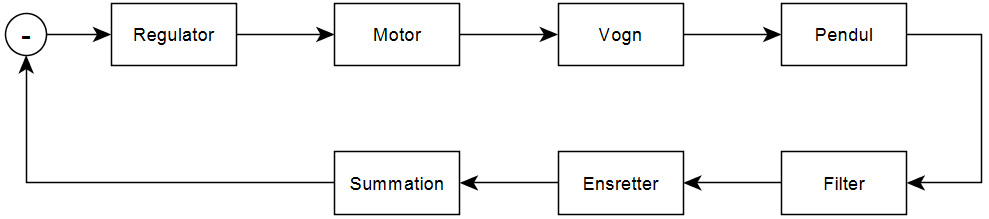
\includegraphics[width=.8\textwidth]{billeder/reg_diagram.png}
	\caption{Diagram over alle overførelsesfunktions-blokke i systemet.}
	\label{fig:reg_diagram}
\end{figure}
\FloatBlock 

I figur \ref{fig:reg_diagram} fremgår alle overførelsesfunktioner i hele systemet som skal beskrives.
De enkelte blokke vil her blive opsummeret og gennemgået, startende fra summations punktet i figur \ref{fig:reg_diagram}.

Regulatoren der er det endelige mål, indgår ikke i $H_{ol}$ og bliver derfor sat til $H_{reg} = 1$.   

Motorens dynamik beskrevet i afsnit \ref{sec:sec_motorstyring}, ligning \ref{eq:motor_trans} giver os den elektriske dynamik for motoren
\begin{align}
H_{motor}(s) = 1,6 \cdot \frac{\num{18E-3}s}{\num{18E-3}s +1}
\end{align}

For at kunne beskrive selv vognen, blev der i afsnit \ref{sec:sec_motoroverforelse} udledt ligning \ref{eq:vogn_dynamic_trans}
\begin{align}
H_{vogn}(s) =\frac{0,66}{s} + \frac{1,37}{s^2} 
\end{align}
Under målingerne af vognens dynamik i afsnit \ref{sec:sec_motoroverforelse} kom det frem, at der skulle en hvis strømstyrke til for at få vognen i bevægelse.
Vi vælger derfor kun at medtage den del at dynamikken der ligger inde for det område hvor vognen er i bevægelse og ser derfor bort fra, at vi ikke kan beskrive den dynamik der ligger mellem $-1 \si{\ampere} < I < 1 \si{\ampere}$. 
Således kan dynamikken for vognen forenkles til
\begin{align}
 H_{vogn}(s) = 1,37
\end{align}

For pendulet vil vi anvende $H_{pendul}$ i ligning \ref{eq:h_pendul}.
\begin{align}
H_{pendul}(s) = \frac{1}{Ls^2 - g} 
\end{align}

I afsnit \ref{sec:filter} bliver indgangsfilteret dimensioneret med en resonansfrekvens på $f_0 = 44,557 \si{\kilo\hertz}$, og en forstærkning på $h_0 = 3,5$. 
Selv om indgangsfilteret er designet som et båndpas-filter, vil vi i reguleringen anse det som et lavpas-filter.
Således vil overførelsesfunktionen for filteret kunne forenkles til 
\begin{align}
H_{filter}(s) = \frac{H_0}{(2 \pi f_0)^{-1}s +1} = \frac{3,5}{\num{3.571E-06}s +1}
\end{align}

Ligeledes kan den designede ensretning af feedback signalet efter filteret, beskrives som et lavpas-filter.
Den beregnede tidskonstant $\tau = 470 \si{\micro\second}$ angiver tidskonstanten i dynamikken for ensretningen og kan beskrives som
\begin{align}
H_{ensretter}(s) = \frac{1}{\tau s +1} = \frac{1}{\num{4.70E-4}s +1}
\end{align} 

Endeligt samles de to indkommende signaler fra sensor spolerne i et summationspunkt, beskrevet i afsnit \ref{sec:summa}.
Her er dynamikken i den anvendte instrumenteringsforstærker udeladt og kun signalforstærkningen er medtaget.
\begin{align}
H_{summa}(s) = 4,5
\end{align}  

\subsection{Forhold mellem sensor signal og pendul vinkel}
Det er i dimensioneringen af vores reguleringssystem, vigtigt at kende forholdet mellem pendulets vinken $\theta$ og signalstyrken på indgangen til filteret.
Ved at video optage pendulet i frit fald, samtidig med at signalet fra den ene af modtagerspolerne blev optaget på et oscilloskop, er det muligt at plotte dette forhold i en graf. Resultatet ses i figur xx.
Vinklen af pendulet blev målt ved videoanalyse i Tracker, hvor der i figur \ref{fig:pendul_fald_vid} er vist et billede fra video optagelsen.
Dataerne fra to forskellige kilder blev efterbehandlet i Matlab og synkroniseret ud fra slutpunktet for faldet.
\begin{figure}[h!]
	\centering
	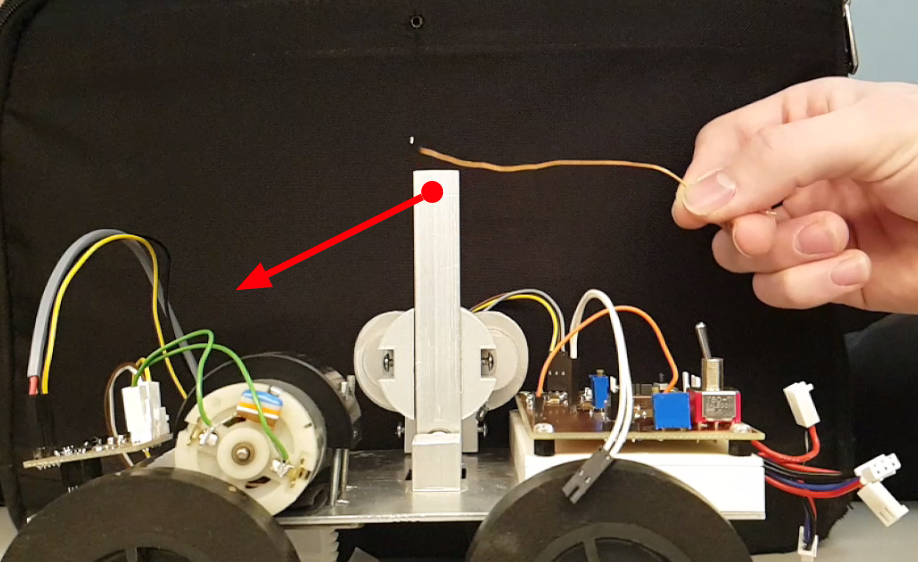
\includegraphics[width=.6\textwidth]{billeder/pendul_fald_vid.png}
	\caption{Enkelt billed fra video optagelsen til måling af forhold mellem pendul vinkel og signal. Rød pil viser frit falds retning af pendul.}
	\label{fig:pendul_fald_vid}
\end{figure}
\FloatBlock
Som det ses ud fra resultaterne i figur \ref{fig:pendul_fald_res}, er forholdet mellem pendulets vinkel og signalet efter signal behandlingen ikke lineært.
Dette betyder at der omkring pendulet arbejdspunkt ved nul grader, skal findes en lineær model.  

\begin{figure}[h!]
	\centering
	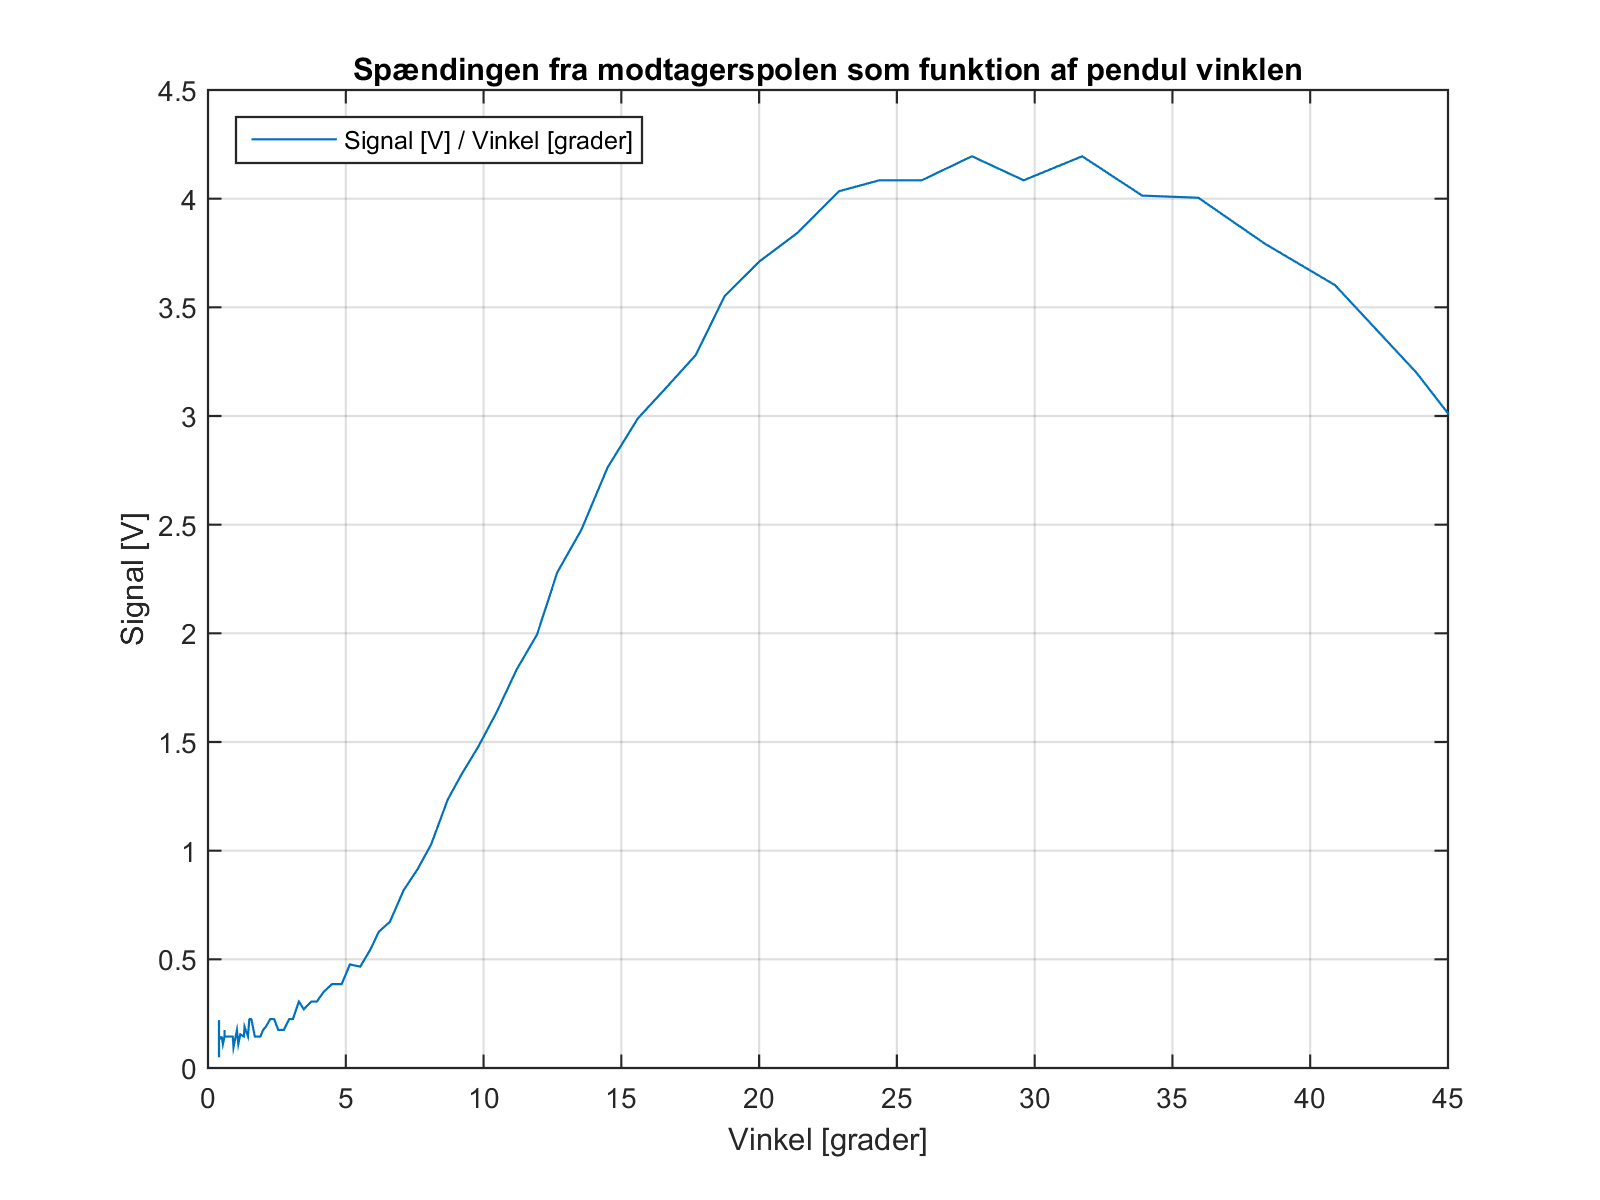
\includegraphics[width=.7\textwidth]{billeder/pendul_fald_res.png}
	\caption{Forholdet mellem signalspændingen fra modtagerspolen og pendulet vinkel.}
	\label{fig:pendul_fald_res}
\end{figure}
\FloatBlock
Der viste sig desværre at være problemer med forsyningen til afsenderspolen, således at det målte signal ikke havde den tiltænke styrke.
Efter tilretning af forsyningen skal denne måling foretages igen, og den korrekte værdi bruges.
Desværre var det ikke muligt at nå indenfor afsatte tidsramme, så i de efterfølgende beregninger anvendes et estimat.

For at opnå bedst følsomhed af sensoren, vil et optimalt signal til vinkel være at have et spændingsinterval på signalet mellem $0-5\si{\volt}$ for $10^{\circ}$ 
\begin{align}
5\si{\volt} = \frac{\pi}{180} \cdot 10^{\circ} \Rightarrow \frac{\si{\volt}}{rad} = \frac{\pi}{180} \cdot 2 = 0,0349
\end{align}


\subsection{Dimensionering og valg af regulator}
Med de forgående beskrivelser af overførelsesfunktionerne i figur \ref{fig:reg_diagram} , er $H_{OL}$ for systemet bestemt til
\begin{align}
H_{OL} &= H_{regulator} \cdot H_{motor} \cdot H_{vogn} \cdot H_{pendul} \cdot H_{filter} \cdot H_{ensretter} \cdot H_{summa} \\
&= \frac{7,533}{\num{5.035e-10} s^4 + \num{1.421E-4} s^3 + 0,3 s^2 - \num{4.65E-3 }s - 9,82}
\end{align} 
$H_{OL}$ er afbilledet i figur \ref{fig:reg_bode_all} som den røde kurve.
Her ses det at for hele frekvensområdet, er fasedrejningen $180^{\circ}$ eller derover.
\begin{figure}[h!]
	\centering
	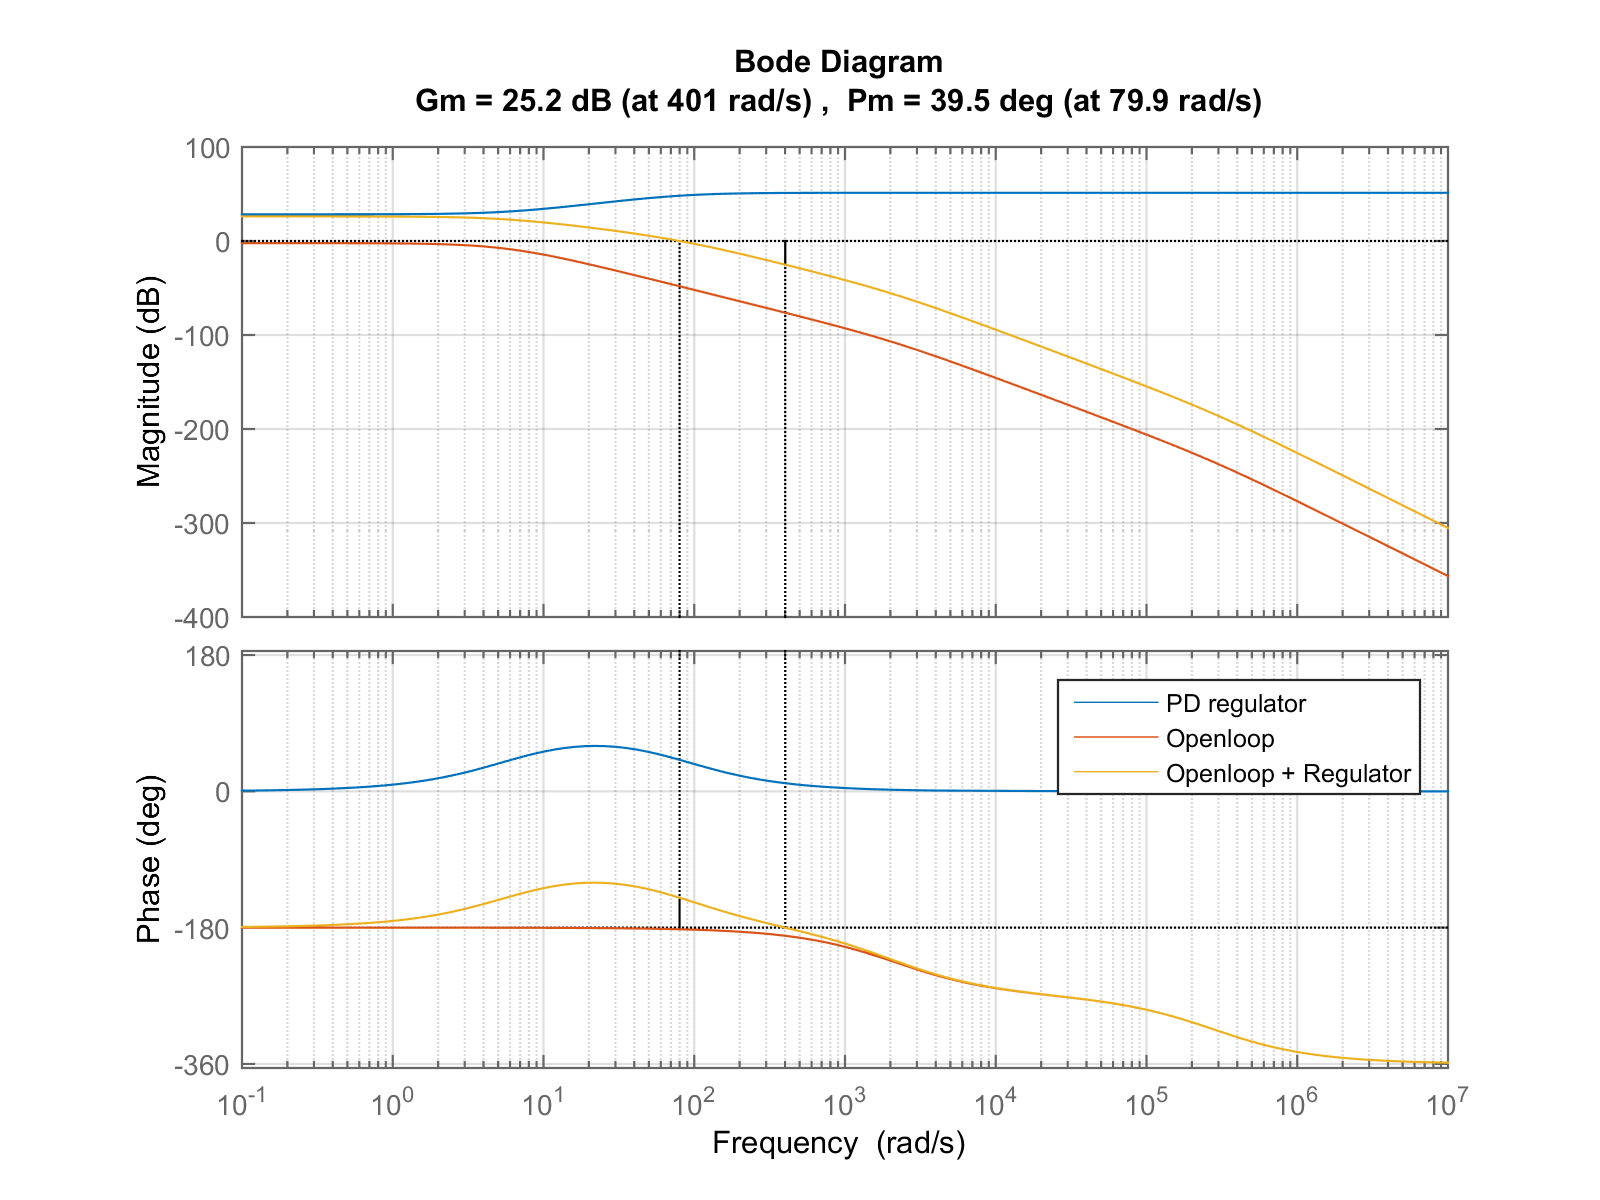
\includegraphics[width=1\textwidth]{billeder/reg_bode_all.png}
	\caption{Bodeplot for $H_{OL}$ (rød), Regulatoren (blå) og $H_{OL}$ med regulator (gul).}
	\label{fig:reg_bode_all}
\end{figure}
\FloatBlock 
Det vælges derfor at dimensionere regulatoren som en P-lead regulator (PD).
Denne type regulator vil kun give et positivt fase bidrag, og vil derfor egne sig særligt godt her.
PD regulatoren kan beskrives som \cite[s.276, (6.7)]{Reg2015}
\begin{align}
G_c(s) = K_p \frac{\tau_d s + 1}{\alpha \tau_d s + 1} \quad, \quad \alpha < 1  \label{eq:reg_gc}
\end{align}	
Her er $G_c(s)$ det samme som $H_{regulator}$. 
Først skal $\alpha$ bestemmes ud fra den ønskede fase drejning $\varphi_m$. Som udgangspunkt vil en fasedrejning på $\varphi_m = 60^{\circ}$ var ønskeligt \cite[s. 278]{Reg2015}
\begin{align}
\alpha = \frac{1 - \sin{\varphi_m}}{1 + \sin{\varphi_m}} = \frac{1 - \sin{60^{\circ}}}{1 + \sin{60^{\circ}}} = 0,0718
\end{align}
PD-regulatorens krydsfrekvens $\omega_m$ skal nu findes til det punkt hvor den ønskede fasedrejning skal bruges til at kompensere og stabilisere systemet.
Amplituden $A_m$ for regulatoren kan bestemmes ved \cite[s. 277, fig. 6.21]{Reg2015}
\begin{align}
A_m = 20 \log \left(\frac{1}{\sqrt{\alpha}}\right) =  20 \log \left(\frac{1}{\sqrt{0,0718}}\right) = 26,3392 \si{\decibel}
\end{align}
$\omega_m$ kan nu findes ud fra det uregulerede $H_{OL}$ plot hvor $|H_{OL}| = -A_m$.
Her bliver $\omega_m$ aflæst i figur \ref{fig:reg_bode_all} til $22,1 \si{\radian\per\second}$. 
Nu kan $\tau_d$ bestemmes som \cite[s. 279, (6.13)]{Reg2015}
\begin{align}
\tau_d = \frac{1}{\omega_m\sqrt{\alpha}} = \frac{1}{22,1 \si{\radian\per\second}\sqrt{0,0718}} = 0,1689 \si{\second}
\end{align}

Den endelige PD-regulator har således overførelsesfunktionen
\begin{align}
H_{regulator}(s) = 26,3392 \frac{0,1689 s + 1}{0,0121 s + 1}  \label{eq:reg_pd_final}
\end{align}	


\subsection{Simulering af reguleret system}
I Matlab er det samlede system blevet designet i SimuLink, for at efterprøver om regulatoren kan sørge for at stabilisere system som tiltænkt.
I figur \ref{fig:transfunc_sim} ses den samlede simulering model.
Med i simuleringen er der også taget de fysiske begrænsninger der er ved fx. udgangsspændingen fra operationsforstærkere i regulatoren, og de strømbegrænsninger der findes for motor og vogn dynamikken.
Endeligt har simuleringen fået tilføjet en tilfældig pulsgenerator, som tilføjer tilfældige forstyrrelser under simuleringen.
Da det ønskes at sætte fokus på pendul vinklen $\theta$ i simulerings resultattern, er regulator signalet og forstyrrelsen blevet faktoriseret, således at detaljerne for pendul vinklen ikke bliver udvisket.
Resultatet af simuleringen kan ses i figur \ref{fig:system_sim_stimuli}.
\begin{figure}[h!]
	\centering
	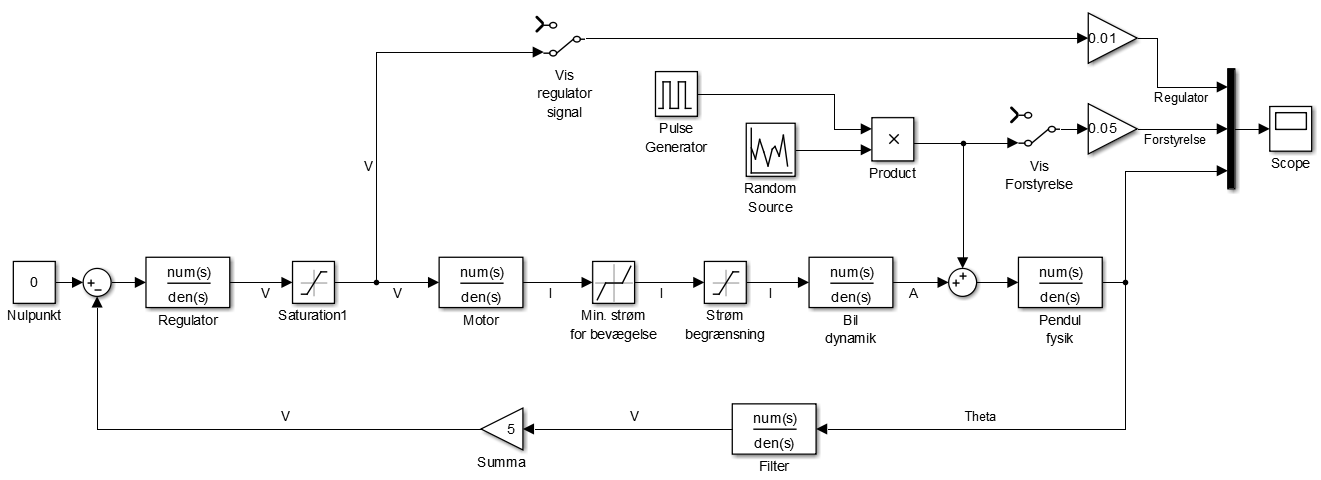
\includegraphics[width=1\textwidth]{billeder/transfunc_sim.png}
	\caption{Simulink simulering model af det samlede system.}
	\label{fig:transfunc_sim}
\end{figure}


\begin{figure}[h!]
	\centering
	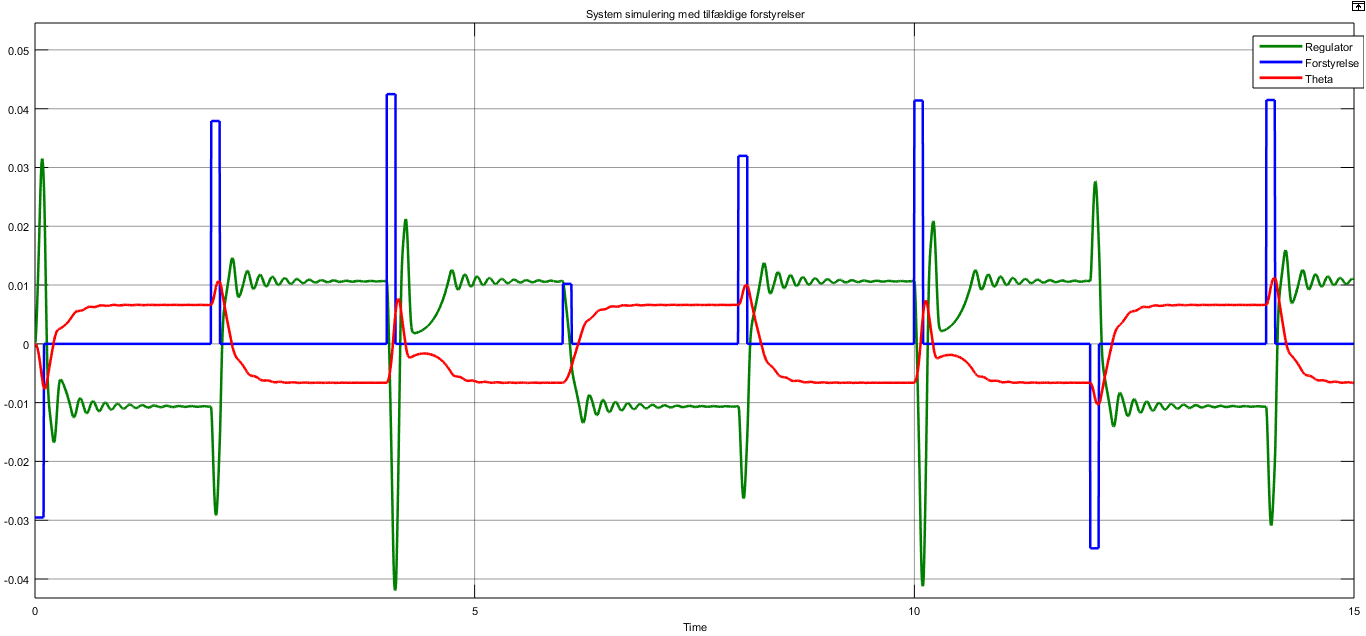
\includegraphics[width=1\textwidth]{billeder/system_sim_stimuli.png}
	\caption[Systemsimulering med tilfældige forstyrrelser.]{Systemsimulering med tilfældige forstyrrelser. Pendul vinkel (rød), Forstyrrelse (blå) og Regulator signal (grøn)}
	\label{fig:system_sim_stimuli}
\end{figure}
\FloatBlock 

\subsection{Implementering af regulator}
\begin{figure}[h!]
\centering
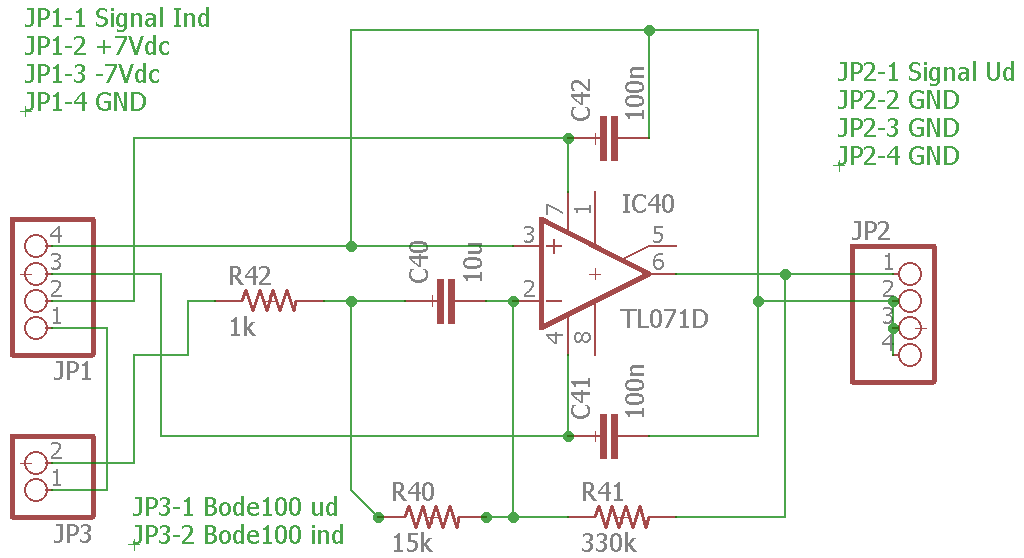
\includegraphics[width=.8\textwidth]{billeder/pd_schematic.png}
\caption{Kredsløbsdiagram af den implementerede PD regulator.}
\label{fig:pd_schematic}
\end{figure}
Med den endelige PD-regulator i ligning \ref{eq:reg_pd_final} og med de ovenstående værdier $K_p$, $\tau_d$ og $\alpha$ kan denne realiseres \cite[s. 349]{Reg2015} som
\begin{align}
K_p = \frac{R_{21}}{R_{20} + R_{22}} \quad , \quad \tau_d = R_{22}C_{20} \quad, \quad \alpha\tau_d = \frac{R_{20} R_{22} C_{20}}{R_{20} + R_{22}}
\end{align}
hvor parameterne fastsættes iht. kredsløbet i figur \ref{fig_pd_schematic}.
Ved at fastsætte $R_{22}$ til $1\si{\kilo\ohm}$ kan resten af værdierne bestemmes til
\begin{align}
R_{20}=12,9\si{\kilo\ohm} \quad, \quad R_{21}=367\si{\kilo\ohm} \quad, \quad C_{20} = 13\si{\micro\farad}
\end{align}

\subsection{Måling af systemet overførelsesfunktion med Bode 100}
Afslutningsvis blev det forsøgt at lave en brugbar måling af systemets overførelsesfunktion med Bode 100\footnote{OMNICRON Lab Bode 100 - \url{https://www.omicron-lab.com/bode-100/}}, når vognen med pendul var i stabil drift.
Det var meget svært at få brugbare data som kunne bruges til verifikation af den teoretisk opstillede model af systemet.
Resultatet er her medtaget i figur \ref{fig:bode100}, men vil ikke anvendes yderligt.
\begin{figure}[h!]
	\centering
	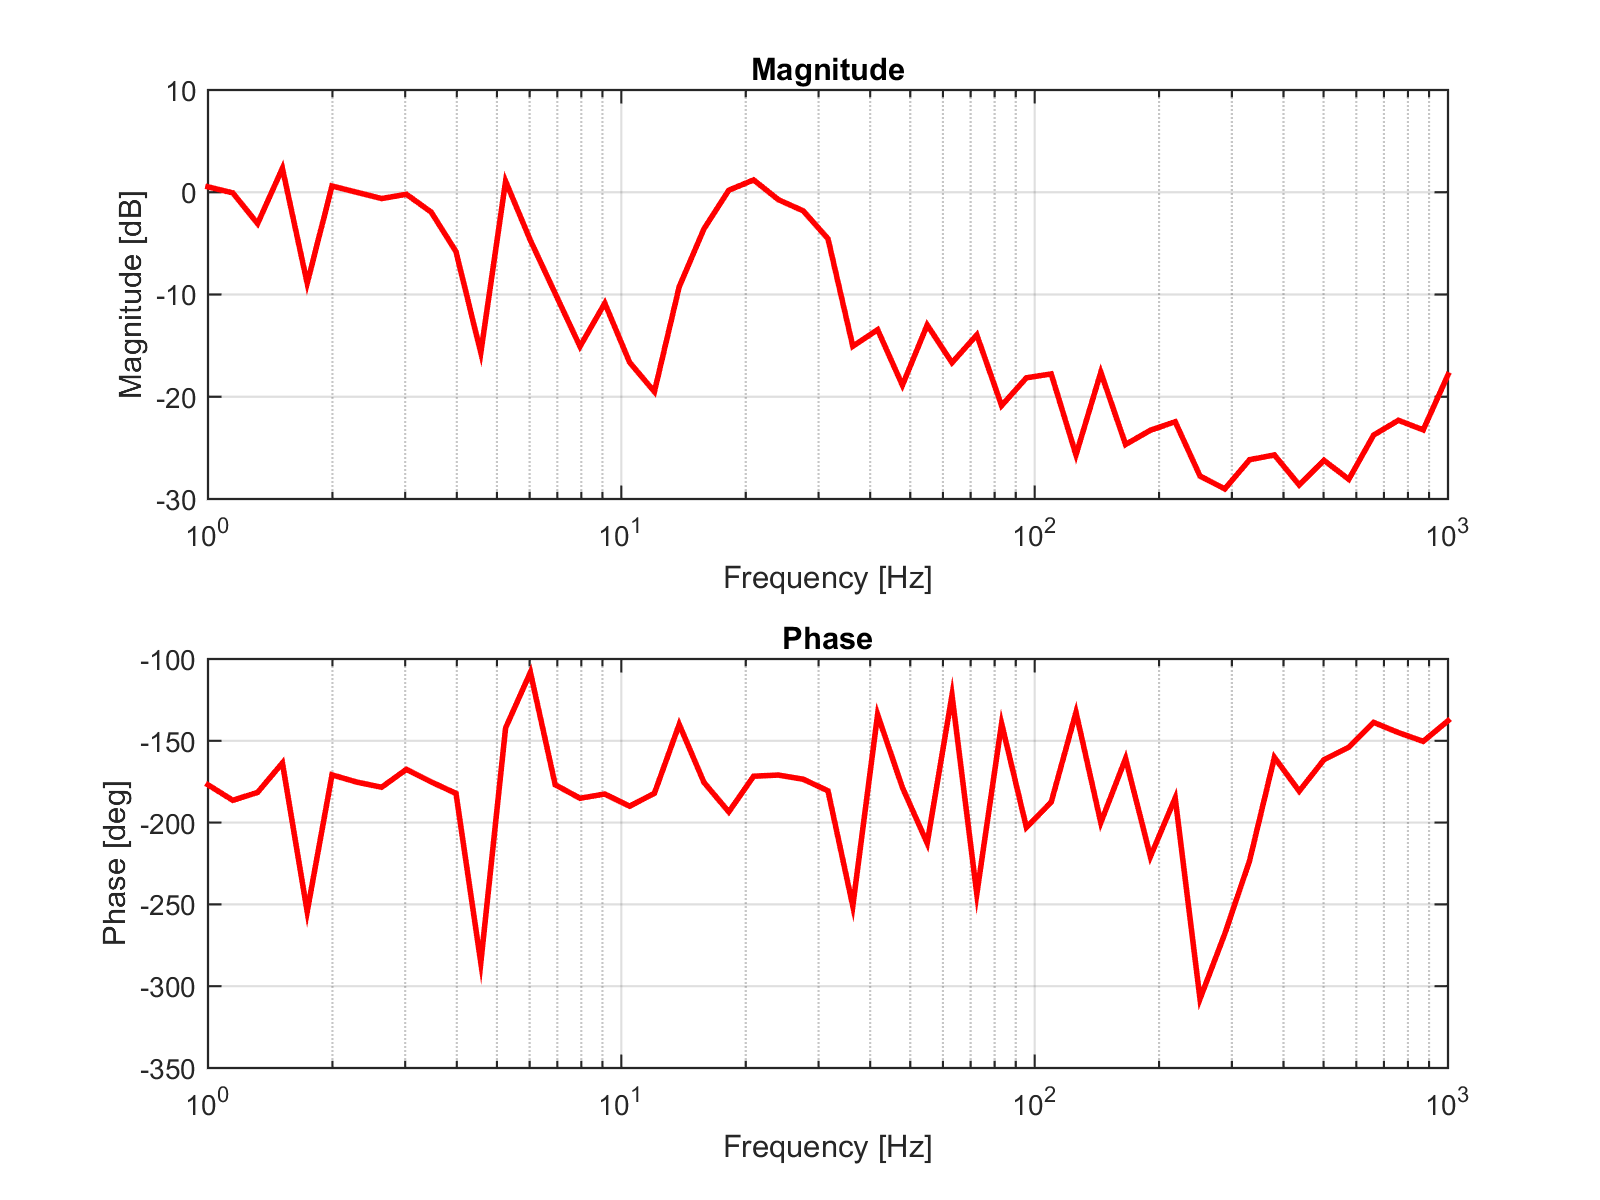
\includegraphics[width=.8\textwidth]{billeder/bode100.png}
	\caption{Måling af system med Bode 100.}
	\label{fig:bode100}
\end{figure}

\section{Opsamling af regulering og motorstyring}
Motorstyringen der skal bruges på vognen er blevet realiseret og dimensioneret og efterfølgende modificeret, så motor på vognen kan forsynes med en stor nok strøm der giver vognen den ønskede bevægelse.
Derudover viste det sig også muligt at bestemme overførelsesfunktionerne, ikke kun for pendul og den elektriske del af motoren, men også for alle andre dele af systemet, således at det blev muligt at designe og dimensionere en regulator der gjorde systemet af pendul og vogn stabilt.
Det må konkluderes at tilgangen har været tilstrækkeligt, da det endelige produkt viste sig at være stabilt.




